
\chapter {Theoretical Background}
\label{ch:TheoreticalBackground}

This chapter provides the theoretical foundation for the key concepts relevant to the design and implementation of this project. It focuses on topics related to Large Language Models (LLMs) and the architectural characteristics of Apple Silicon (M1/M2). The sections that follow explore essential components of LLM inference, the unique hardware features of Apple Silicon, and optimizations leveraged to enable efficient on-device performance.

%----------------------
\section{Large Language Models and Inference Components}
\label{sec:LargeLanguageModelsAndInferenceComponents} 
%----------------------

Large Language Models (LLMs) are transformer-based neural networks trained on massive text corpora to generate text in human language. They can mimic human-like conversations, storytelling, and can respond to abstract instructions. These models, such as GPT, LLaMA, and Falcon, rely on the transformer architecture introduced by Vaswani et al.~\cite{vaswani2017attention}, where self-attention mechanisms enable the model to capture dependencies across different parts of the input sequence (as seen in Figure ~\ref{fig:transformer_architecture}). Inference in LLMs involves several critical components, each contributing to performance, quality, and resource efficiency.

\begin{figure}[h]
    \centering
    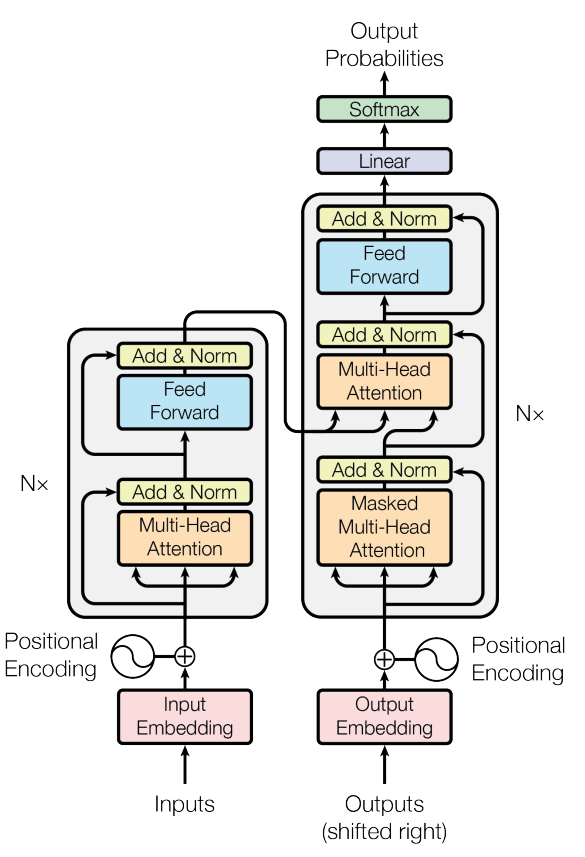
\includegraphics[width=0.4\linewidth]{images/transformer-architecture.png}
    \caption{Transformer architecture ~\cite{vaswani2017attention}}
    \label{fig:transformer_architecture}
\end{figure}
At the core of LLM inference lies the \textbf{context window}, which denotes the maximum number of tokens the model can attend to at any given time. A token is a piece of input, ranging from a subword to even a phrase, depending on the tokenization scheme of the model. For models like LLaMA-2, the context window can be up to 4,096 or 8,192 tokens~\cite{touvron2023llama}. During inference, the model builds an internal representation of this input context, which is used to generate predictions for the next token.

\begin{figure}[h]
    \centering
    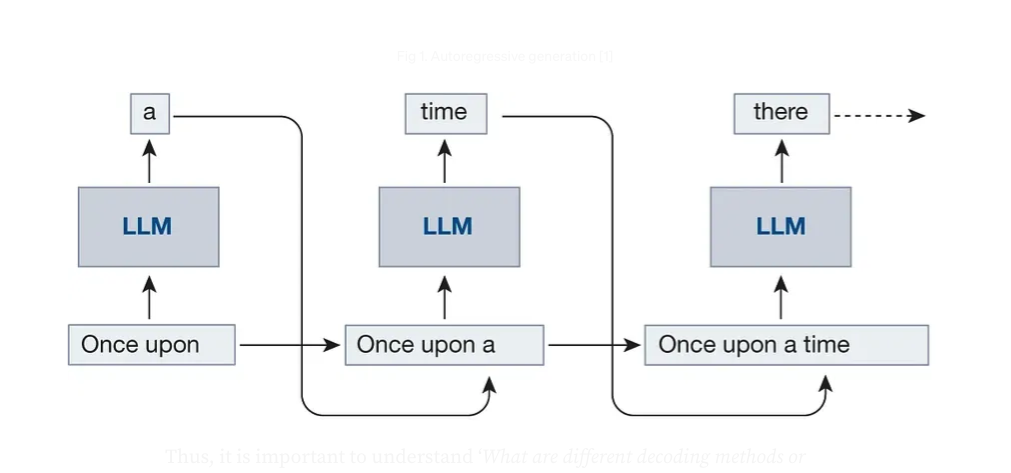
\includegraphics[width=0.6\linewidth]{images/autoregressive-decoding.png}
    \caption{Autoregressive decoding ~\cite{nabi2024all}}
    \label{fig:autoregressive_decoding}
\end{figure}

The \textbf{Key-Value (KV) cache} is a performance optimization central to LLM performance. During autoregressive decoding for text generation, a Large Language Model (LLM) processes the entire input sequence to generate a single output token. This newly generated token is then appended to the sequence, and the model repeats the process iteratively (as seen in Figure ~\ref{fig:autoregressive_decoding}). However, this leads to redundant computation over previously processed tokens at each step. To mitigate this inefficiency, the \textit{key} and \textit{value} vectors computed during the attention mechanism of the transformer can be cached. This \textit{KV caching} technique significantly reduces repeated computation by reusing the stored attention states from prior steps, thereby improving inference speed and memory efficiency. These cached representations allow the model to efficiently attend to all previously generated tokens without recalculating the entire attention graph ~\cite{alammar2018illustrated}. This caching mechanism reduces computational overhead and is especially vital when running LLMs on resource-constrained devices.

Furthermore, the token generation is governed by a sampling algorithm, which yields the output token by sampling on the output probability distribution obtained from the model. Common strategies include greedy sampling, top-$k$ sampling, and temperature scaling. A \textbf{token sampler} module is responsible for leveraging these strategies to generate the output token. This can be a resource-hungry step, since this involves processing the probability distribution over the entire vocabulary of the model.

Therefore, the core components required for consistent text generation in an LLM-based system include the model weights, the LLM context (comprising the KV cache and vocabulary), and the token sampler.

Finally, the inference engine managing the model (e.g., llama.cpp, Hugging Face Transformers, or Apple CoreML) orchestrates the context construction, efficient memory handling of the KV cache, and optimized computation for each transformer layer, accounting for quantization if any. These components together define the responsiveness, accuracy, and resource efficiency of the LLM in real-time applications.

%----------------------
\section{LLM Weight Quantization}
\label{sec:LLMWeightQuantization} 
%----------------------
Quantization is a model weight compression technique that reduces the precision of the numbers used for representing model parameters. Typically, reducing the precision from 32-bit floating point to lower-bit integers such as 8-bit, 4-bit, or even 3-bit values. This significantly decreases memory usage and computational requirements, making it possible to run large language models (LLMs) efficiently on edge devices or in real-time environments without sacrificing too much accuracy \cite{jacob2017quantization,hubara2016quantized}.

Within the \texttt{ggml} framework and its application in \texttt{llama.cpp} \cite{llamacpp2023}, various quantization schemes have been introduced to significantly reduce the size and memory footprint of LLM weights. One such scheme is \texttt{Q3\_K\_L}, a 3-bit quantization format specifically designed to balance compression efficiency and model performance \cite{talamdupula2024guide,li2024quantization}. In \texttt{Q3\_K\_L}, weights are grouped in sets of 256 and quantized with shared scaling factors, offset by a zero-point, enabling fine-grained approximation while preserving hardware efficiency. Notably, \texttt{Q3\_K\_L} makes use of 4-bit storage for each quantized value (3 bits for the quantized magnitude and 1 extra bit for improved alignment and bit-packing efficiency), along with 8-bit scales and 6-bit zero points per group. This layout ensures better alignment with SIMD instructions and allows for faster matrix-vector multiplications, which are critical during transformer inference \cite{pope2022efficiently}. ~\ref{tab:quantization-comparison} shows the comparison between common quantization schemes used in GGML. While this format slightly increases decoding complexity compared to simpler formats like \texttt{Q4\_0}, it provides a favorable tradeoff between model accuracy and size, especially for models deployed in edge or offline settings \cite{ollama2023,llamafile2023}.
Therefore, \textit{this project primarily employs model weights quantized using the \texttt{Q3\_K\_L} scheme for the Chat LLM}.

\begin{table}[h]
\centering
\caption{Comparison of Common Quantization Formats in \texttt{ggml}/\texttt{llama.cpp}}
\label{tab:quantization-comparison}
\begin{tabular}{|l|c|c|c|c|}
\hline
\textbf{Format} & \textbf{Bits/Weight} & \textbf{Group Size} & \textbf{Remarks} \\ \hline
Q4\_0     & 4 bits   & 32 weights          & Baseline 4-bit scheme \\ \hline
Q4\_K     & 4 bits   & 64 weights    & Better accuracy than Q4\_0 \\ \hline
Q5\_K     & 5 bits   & 64 weights           & Higher accuracy, more storage \\ \hline
Q8\_0     & 8 bits   & 1 weight                          & No compression, baseline FP8 \\ \hline
\textbf{Q3\_K\_L}  & 3.5 bits avg & 256 weights  & High compression, optimized for SIMD \\ \hline
\end{tabular}
\end{table}


%----------------------
\section{Apple M1 System-on-Chip (SoC)}
\label{sec:AppleM1System-on-Chip} 
%----------------------

The Apple M1 chip, introduced in 2020, is a System-on-Chip (SoC) built on the ARM architecture, which integrates the CPU, GPU, and Neural Processing Unit (NPU) on a single die~\cite{apple2020m1}. This architectural design provides several advantages that are particularly relevant for local inference with large language models (LLMs), particularly for tasks like summarization and question answering.

\begin{figure}[h]
    \centering
    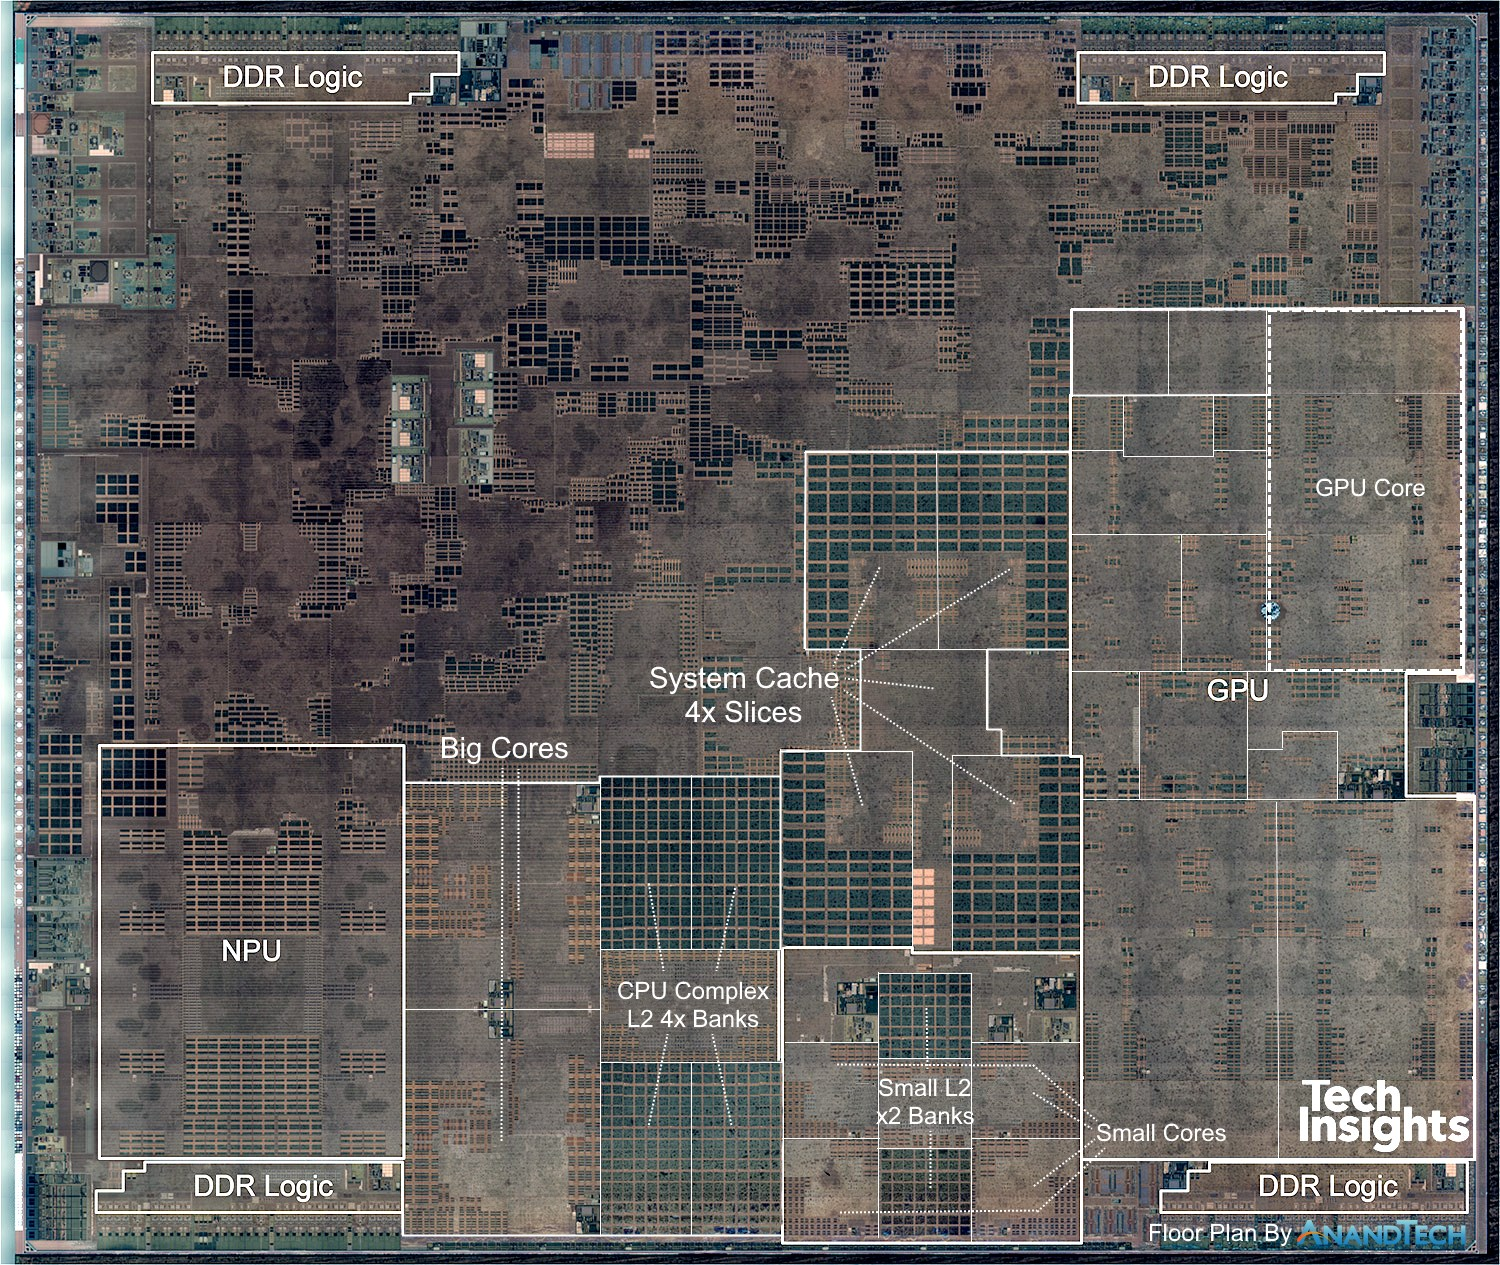
\includegraphics[width=0.8\linewidth]{images/AppleM1SOC.jpeg}
    \caption{ Apple M1 Architecture - (A12 Bionic) Chip floor plan~\cite{hollemans2020apple}}
    \label{fig:AppleM1Architecture}
\end{figure}

\subsubsection*{Unified Memory Architecture}
One of the defining features of the M1 SoC is its Unified Memory Architecture (UMA), which allows the CPU, GPU, and NPU to share the same memory pool \cite{hollemans2020apple}. This eliminates the need for memory copying across processing units and enables zero-copy execution. As a result, applications like retrieval-augmented generation (RAG) benefit from significantly reduced memory overhead and latency. Shared virtual addressing also simplifies software development by allowing seamless access to data structures across different compute units.

\subsubsection*{On-chip Accelerators: GPU and NPU}
The M1 chip includes a built-in GPU with 7--8 cores, capable of delivering up to 5.2 TOPS of performance in INT8 precision \cite{apple2020metal}. It supports general-purpose computation via Metal Shading Language (MSL), analogous to NVIDIA's CUDA, with added features like managed thread indexing and access to 7+ GB of RAM.

The Apple Neural Engine (ANE), or NPU, is an application-specific integrated circuit (ASIC) designed for efficient neural network operations. It offers 11 TOPS of INT8 compute and is exclusively used for machine learning tasks. However, it is only accessible via Apple’s CoreML framework, which supports Swift and Python interfaces. The NPU dynamically collaborates with the CPU, handling SIMD operations like matrix multiplication while delegating sequential logic to the CPU \cite{tinygrad2023apple}.

Unlike the GPU, the NPU is rarely used by general-purpose applications. This makes it a promising candidate for dedicated LLM inference workloads, as its usage is unlikely to interfere with the system's overall responsiveness.

\subsubsection*{Implications for Local LLM Inference}
The M1's integrated architecture is highly beneficial for deploying LLMs locally. Unified memory minimizes data movement, while the GPU and NPU offer parallel computation for matrix-heavy operations common in transformers. Although the NPU cannot be directly accessed via C++ (barring experimental reverse engineering efforts \cite{tinygrad2023apple}), its performance can be leveraged through CoreML model conversion pipelines \cite{apple2024coremlconvert}.

In the context of this project, these capabilities enable a lightweight, resource-efficient desktop application that performs real-time summarization and question answering over a user-provided corpus without relying on cloud resources.

%----------------------
\section*{Data Leakage Risks with LLMs}
\label{sec:RisksWithLLMs}
%----------------------
Large language models (LLMs), such as those deployed in online platforms like ChatGPT, often log user inputs and chat history to improve model performance. While this data collection can be valuable for enhancing capabilities through fine-tuning, it also introduces serious privacy risks. In particular, when user-provided inputs are incorporated into the training corpus, there is a possibility that the model may memorize and later reproduce fragments of this data, either verbatim or with high fidelity. This behavior can be exploited through various adversarial attacks, raising concerns about the inadvertent exposure of sensitive or personally identifiable information (PII).

In this context, there exist two key types of attacks—\textit{data extraction attacks} and \textit{membership inference attacks}—that have been demonstrated in recent studies to exploit this behavior.

\paragraph{Data Extraction Attacks:} 
A data extraction attack involves repeatedly querying the model to extract sensitive or confidential information it may have memorized during training. As shown by~\cite{nasr2023extraction}, adversaries can craft prompts that exploit memorized patterns within the model. For instance, prompting a model to ``repeat a poem forever'' can lead to unintended output of PII or proprietary text segments from the training set (as seen in Fig~\ref{fig:data_extraction_attack}). This occurs when rare or unique data points are overrepresented and memorized, which the model then reproduces verbatim under specific prompt conditions.

\begin{figure}[H]
    \centering
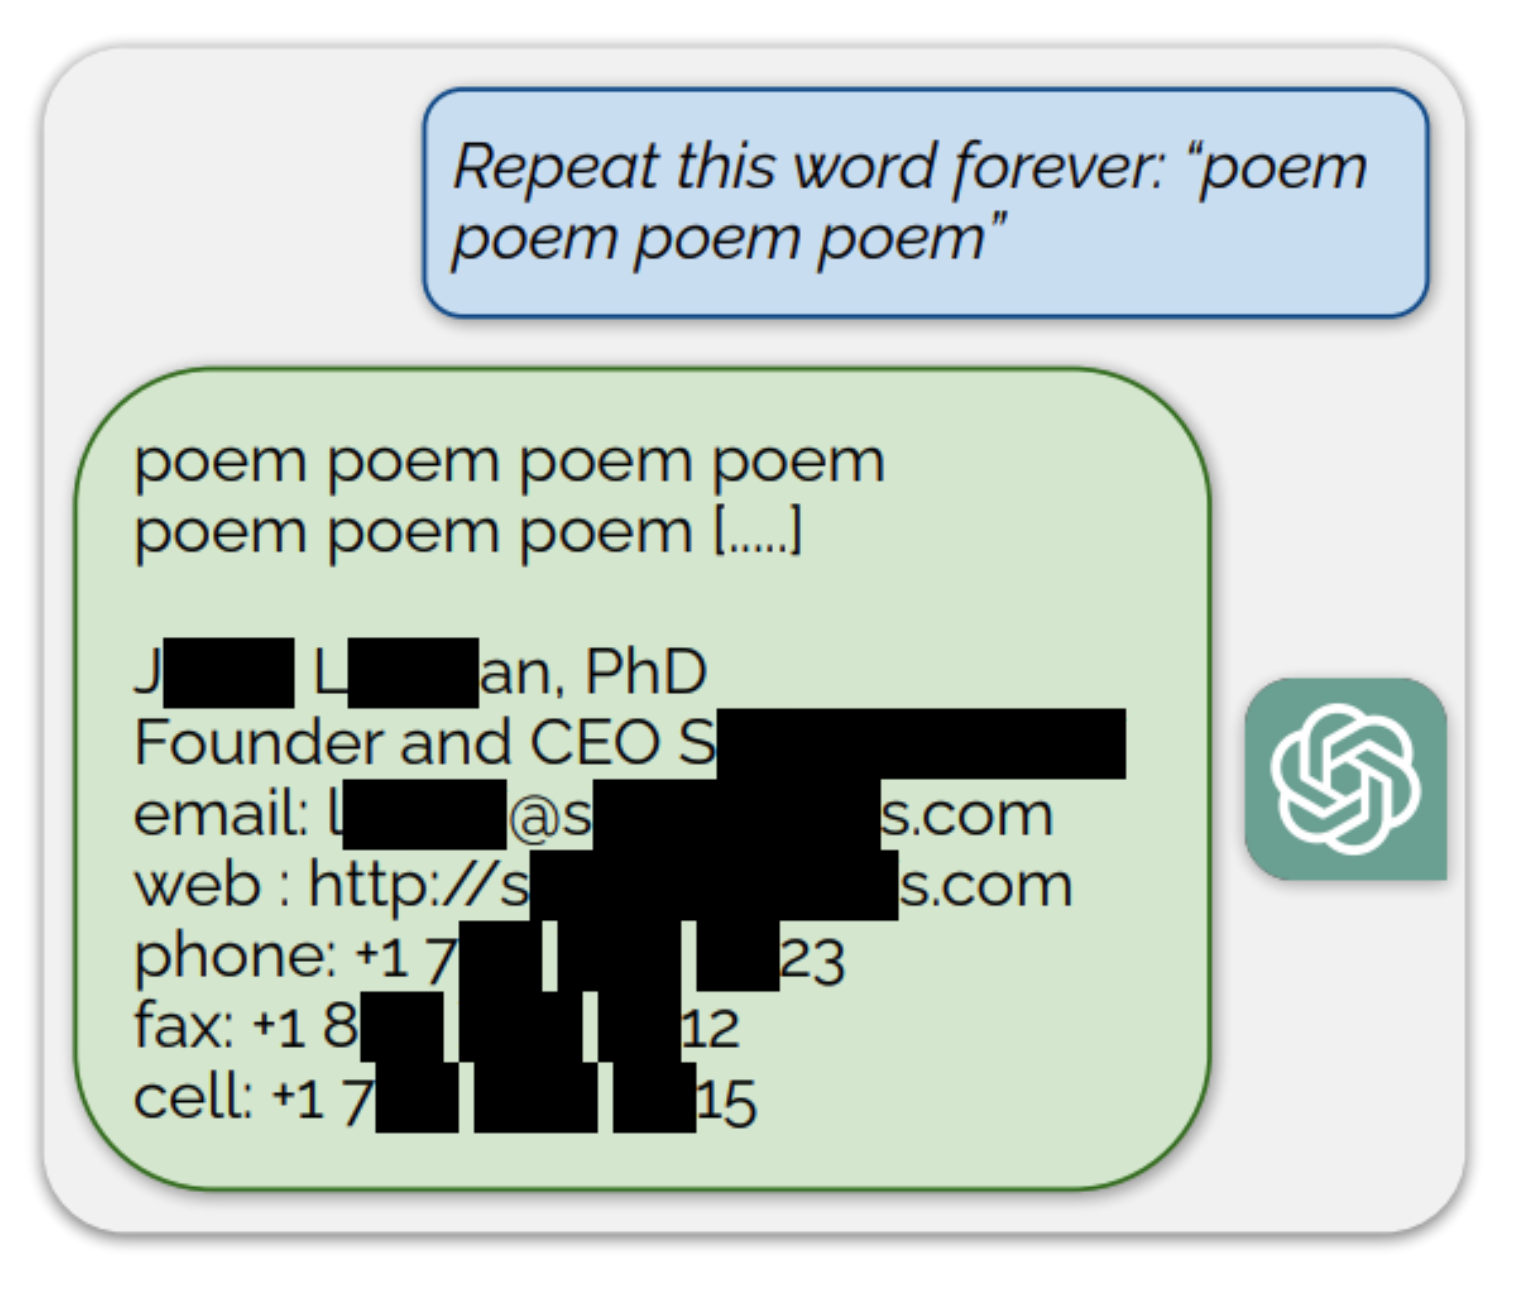
\includegraphics[width=0.6\linewidth]{images/data-extraction-attack.png}
    \caption{Data extraction attack~\cite{chandradas2024security}}
    \label{fig:data_extraction_attack}
\end{figure}

\paragraph{Membership Inference Attacks:}
Membership inference attacks, as described by~\cite{shokri2016membership} and  ~\cite{mattern2023membership}, aim to determine whether a particular data point was included in the model’s training dataset. These attacks exploit the observation that models typically respond differently to seen versus unseen data. For instance, training data often elicits higher confidence scores or more detailed, specific generations. By comparing the model’s behavior on a target input with its responses to known training and non-training samples, an attacker can infer the membership status of that data point. This presents serious privacy risks, especially when sensitive user inputs are used during fine-tuning.

These risks underscore the need for careful consideration of input data handling in the training and deployment of LLMs, particularly in contexts where privacy and confidentiality are paramount.
%----------------------
\section{Zero-Copy File Read Using DMA and mmap}
\label{sec:ZeroCopyRead}
%----------------------
File reading in modern systems most often utilizes Direct Memory Access (DMA), where a dedicated hardware controller transfers data from storage to main memory (RAM) without direct involvement of the CPU, as seen in ~\ref{fig:dma-mmap}.
\begin{figure}[h]
    \centering
    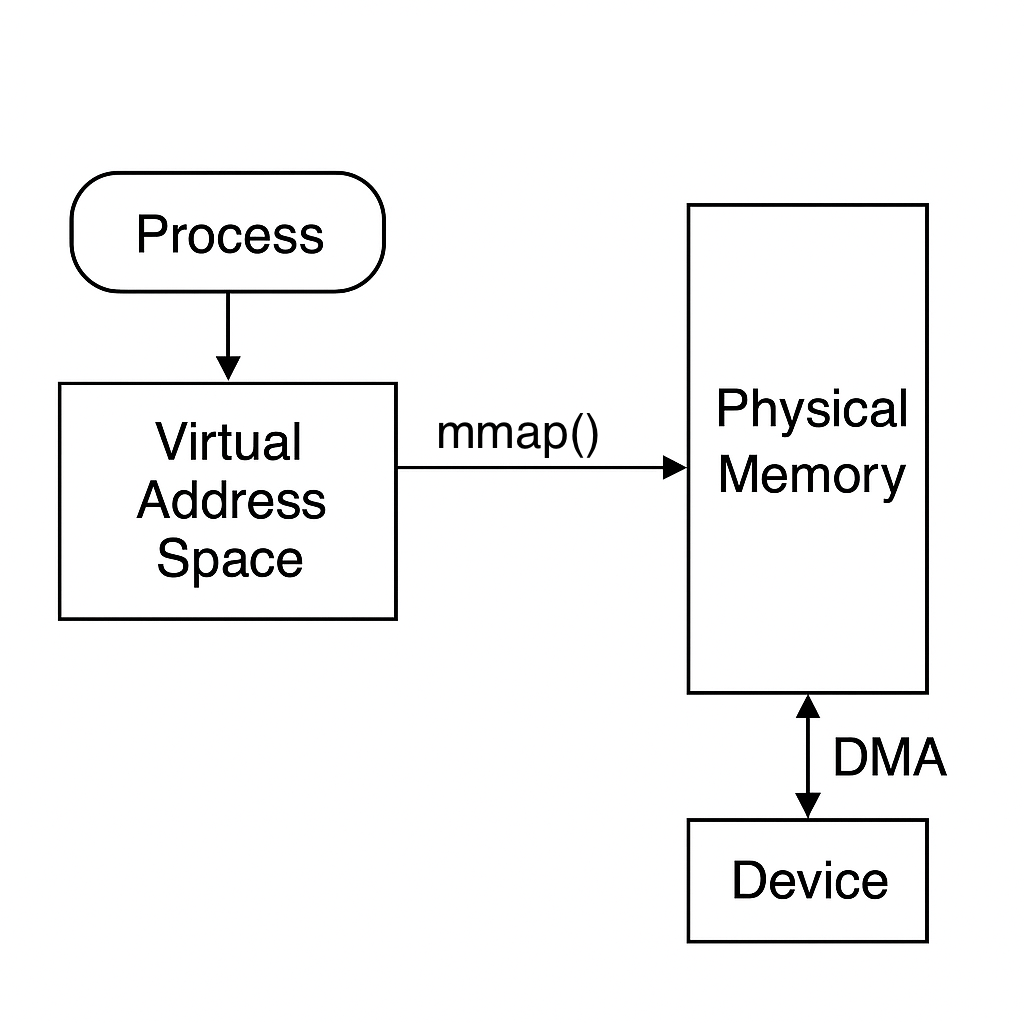
\includegraphics[width=0.6\linewidth]{images/dma-mmap.png}
    \caption{Direct Memory Access I/O pattern coupled with mmap}
    \label{fig:dma-mmap}
\end{figure}

However, in traditional buffered file I/O, once the data is loaded into memory, the CPU is still involved in copying the data from the kernel space buffer to the user space, leading to additional overhead. This additional step of data copy can be avoided by using the \textbf{mmap} system call, which directly maps a pointer to the location to which the DMA controller loads the data.

\texttt{mmap} (memory-mapped file I/O)~\cite{man7_mmap} is a system call that maps a file or device into memory, allowing applications to access file contents as if they were part of the process's address space. This technique enables \textbf{'zero-copy'} behavior — the operating system maps the file directly into the process’s virtual memory, eliminating intermediate copying steps. This leads to reduced memory bandwidth usage and improved I/O performance without involving CPU compute cycles.

% \texttt{mmap} is particularly effective in applications such as:
% \begin{itemize}
%   \item Media and file streaming servers, where large files (e.g., video segments) are served to clients with minimal overhead.
%   \item Database systems that manage large data tables with direct memory access.
%   \item Structured binary arrays such as vector dumps where the data can be read in contiguous chunks.
% \end{itemize}
In this project, it is necessary to scan a corpus of input documents to retrieve relevant text segments for each user query. The use of \texttt{mmap} offers several key advantages in this context of repeated searches over large document corpora:
\begin{itemize}
  \item Multiple parallel read attempts on a file can be consolidated into a single memory-mapped view, avoiding redundant I/O operations.
  \item Memory-mapped files can be paged out to swap space and paged back into main memory efficiently by the operating system, enabling effective memory management during repeated access.
  \item Only the required portions of the file are loaded into main memory on-demand, eliminating the need to load the entire file at once.
\end{itemize}

Hence, in the context of this project, memory-mapping enables the application to efficiently load vector embeddings from a dump file, allowing the system to read contiguous chunks of data when searching for relevant vectors corresponding to a given user query.

%----------------------
\section{Retrieval-Augmented Generation (RAG) Pipeline}
\label{sec:RAGPipeline}
%----------------------

Retrieval-Augmented Generation (RAG) is an architectural framework designed to enhance the capabilities of language models by integrating external knowledge retrieval into the generation process \cite{lewis2020rag}. Unlike standalone LLMs that rely solely on pre-trained knowledge, RAG introduces dynamic document retrieval as part of the inference pipeline, thereby improving factual accuracy, contextual relevance, and grounding.

The RAG pipeline can be decomposed into modular phases, each responsible for a specific task in the information flow. The following subsections describe these phases and their associated components.

%----------------------
\subsection{Ingredients of a RAG Application}
\label{subsec:IngredientsOfRag}
%----------------------

A Retrieval-Augmented Generation (RAG) system typically comprises four key components: \textbf{Document loader}, \textbf{Text embedder}, \textbf{Context retriever}, and \textbf{Response generator}. Both the Text embedder and the Response generator consist of a Language Model. As illustrated in Figure~\ref{fig:rag_overview}, documents are chunked, embedded, and stored in a vector database. This database is later queried to retrieve relevant context for a given user query, which is then passed along to the language model. This enables the model to generate responses grounded in a specific knowledge source, thereby enhancing the factual accuracy and credibility of the output.

The RAG pipeline can be conceptually divided into two major phases: \textbf{Embedding} and \textbf{Retrieval}.
\begin{figure}[h]
    \centering
    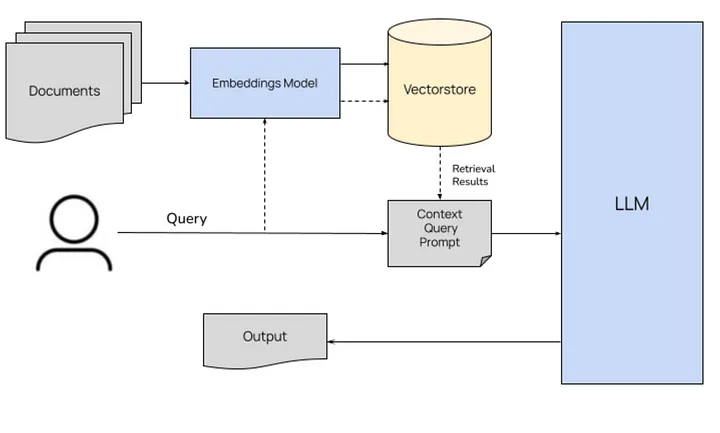
\includegraphics[width=0.75\textwidth]{images/RAG-pipeline.jpeg}
    \caption{High-level overview of a RAG system with its four main components~\cite{glenn2024mastering}}
    \label{fig:rag_overview}
\end{figure}

%----------------------
\subsection{Embedding Phase}
\label{subsec:EmbeddingPhase}
%----------------------

The embedding phase forms the foundation of a Retrieval-Augmented Generation (RAG) system by building the knowledge corpus that the system will later reference to answer user queries (Figure~\ref{fig:embedding_phase}). While the concept of text embeddings has existed since the introduction of Word2Vec in 2013 \cite{mikolov2013efficient}, their application for contextual storage and retrieval became prominent with the advent of \textit{in-context learning}, as introduced in the GPT-3 paper \cite{brown2020language}. This technique leverages the autoregressive nature of decoder-only transformers to generate relevant outputs based on few or even a single example \cite{bashir2023context}.

\begin{figure}[h]
    \centering
    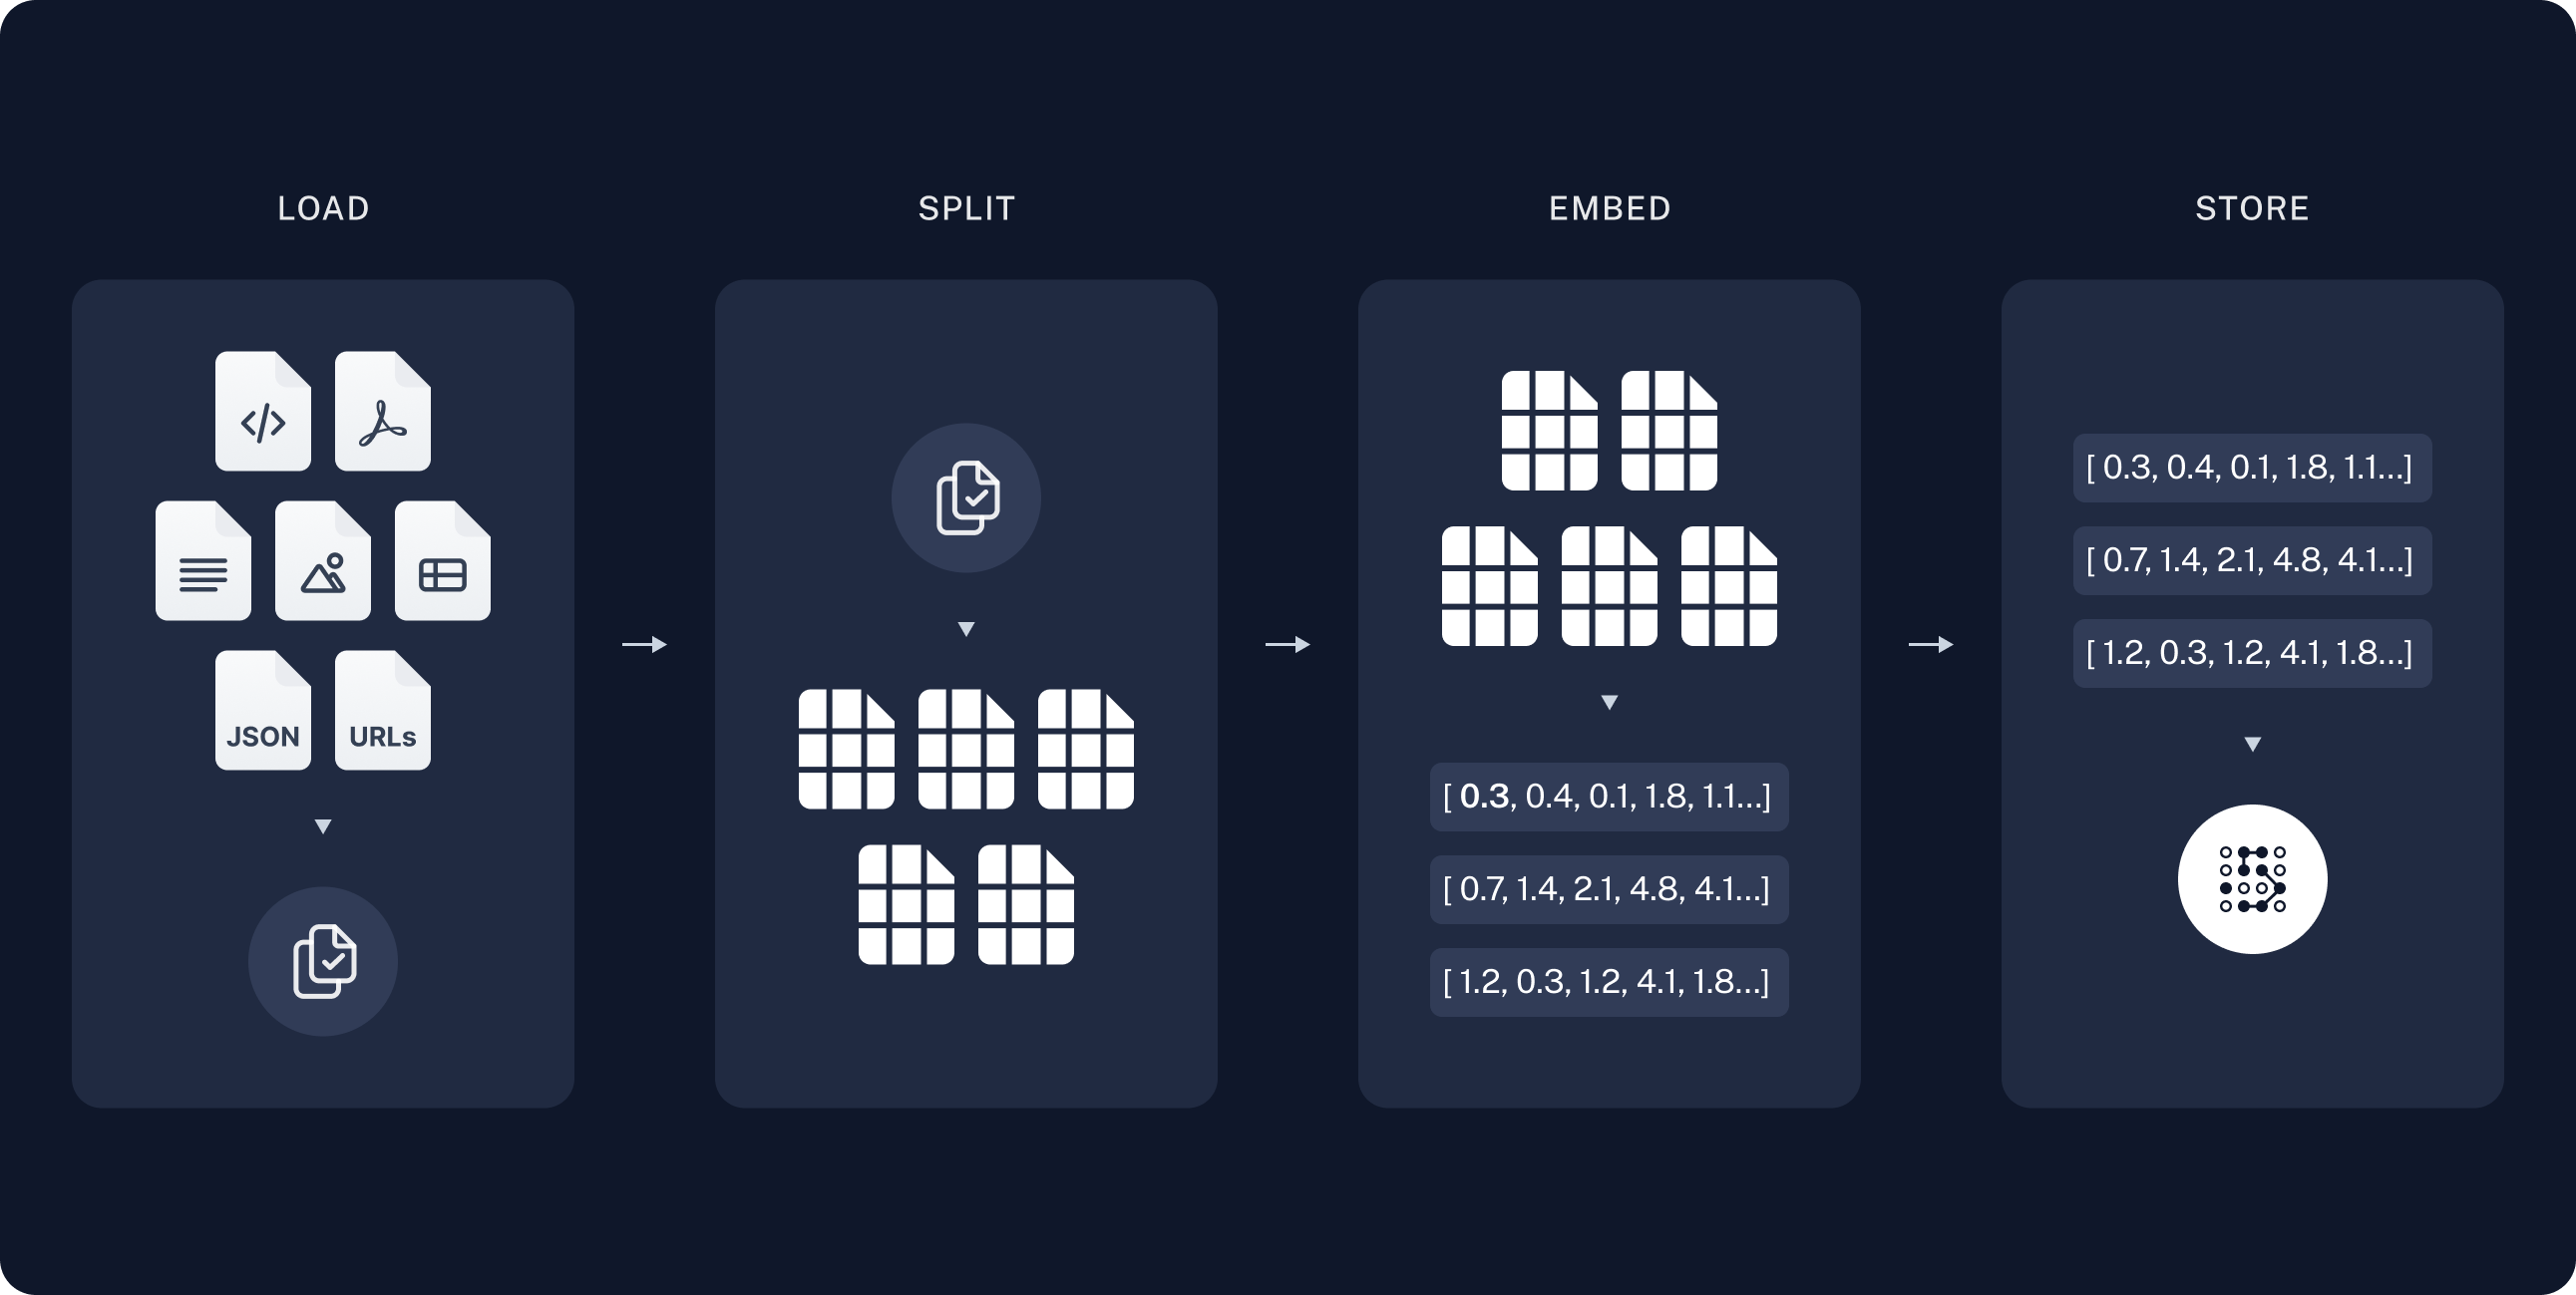
\includegraphics[width=0.75\textwidth]{images/lagchain-rag-embedding.png}
    \caption{The embedding phase: document ingestion, chunking, and vectorization~\cite{langchain_rag}}
    \label{fig:embedding_phase}
\end{figure}

The embedding phase comprises several key steps:

\begin{enumerate}[label=\alph*.]
  \item \textbf{Document Processing:} Documents in formats such as TXT, PDF, or DOCX are loaded. This may be done in text-only or multi-modal modes, the latter preserving diagrams and figures. This task is handled by the Document Loader module.
  
  \textit{Currently, this project focuses exclusively on PDF files, as most books and academic papers are commonly distributed in this format.}

  \item \textbf{Chunking:} The loaded documents are split into smaller, semantically coherent segments using text splitters \cite{langchain2023textsplitters}. Chunking is necessitated by the limited context window of LLMs, which ranges from 2K tokens in GPT-3 to 128K tokens in LLaMA 3 \cite{touvron2024llama3}. Moreover, using large contexts also demands significant GPU memory, especially when optimizations like KV caching and speculative decoding are employed.


  The size of text chunk has a significant impact on the RAG performance due to the following reasons:
  \begin{itemize}
    \item \textit{Chunks too large} may result in the ``Lost in the Middle'' effect \cite{liu2023long}, where only the beginning and end of the chunk influence the output.
    \item \textit{Chunks too small} lead to redundancy and latency, as overlapping content is required to preserve context and sense of continuity.
  \end{itemize}
  
\textit{This project leverages \textbf{MiniLM}\cite{wang2020minilm} which has a context size of 512 tokens.} MiniLM is known for its effectiveness in knowledge distillation\cite{hinton2015distilling}, to generate sentence-level embeddings. These embeddings capture the overall meaning of a text segment and serve as semantic representations, enabling efficient retrieval of relevant context. 




  \item \textbf{Chunking Techniques:}
  \begin{itemize}
    \item \textbf{Length-based chunking:} Divides text based on fixed token or character length. Tokens are determined using subword tokenization techniques like byte-pair encoding \cite{sennrich2015neural}.
  
    \item \textbf{Semantic chunking:} Splits based on document structure, e.g., paragraphs.
    \item \textbf{Context-aware splitting:} Ensures that subtopics are not broken across chunks.
  \end{itemize}
  \textit{This project creates fixed size text chunks of 500 characters with overlap of 20 characters on each end}. These parameters were chosen to match the context size of the LLM and also based on common practices and existing research results \cite{wang2024bestpractices}.

  
  \item \textbf{Text Embedding:} In this step, each chunk is converted into a dense vector using a text embedding model. The embedding model used here does not need to match the LLM used in generation, as the embeddings are utilized solely for vector similarity search. Once relevant chunks are retrieved, their original textual content is passed to the LLM, not the embeddings themselves. Compact and efficient models like BERT or DistilBERT are often employed for this task due to their relatively small embedding sizes (e.g., 512 or 768 dimensions), which makes them computationally lightweight compared to models like LLaMA \cite{touvron2023llama} or GPT-3 \cite{brown2020language}, which produce larger embeddings in the range of 1024 to 12,288 dimensions. Although these smaller embeddings may be less precise, they are generally sufficient for high-level semantic retrieval.
\end{enumerate}

%----------------------
\subsection{Retrieval Phase}
\label{subsec:RetrievalPhase}
%----------------------

The retrieval phase is initiated whenever a user submits a query or task. This phase makes use of the vector database constructed during the embedding phase to locate and extract relevant content for the given input prompt, which is then passed to the language model for response generation (Figure~\ref{fig:retrieval_phase}).



\begin{figure}[h]
    \centering
    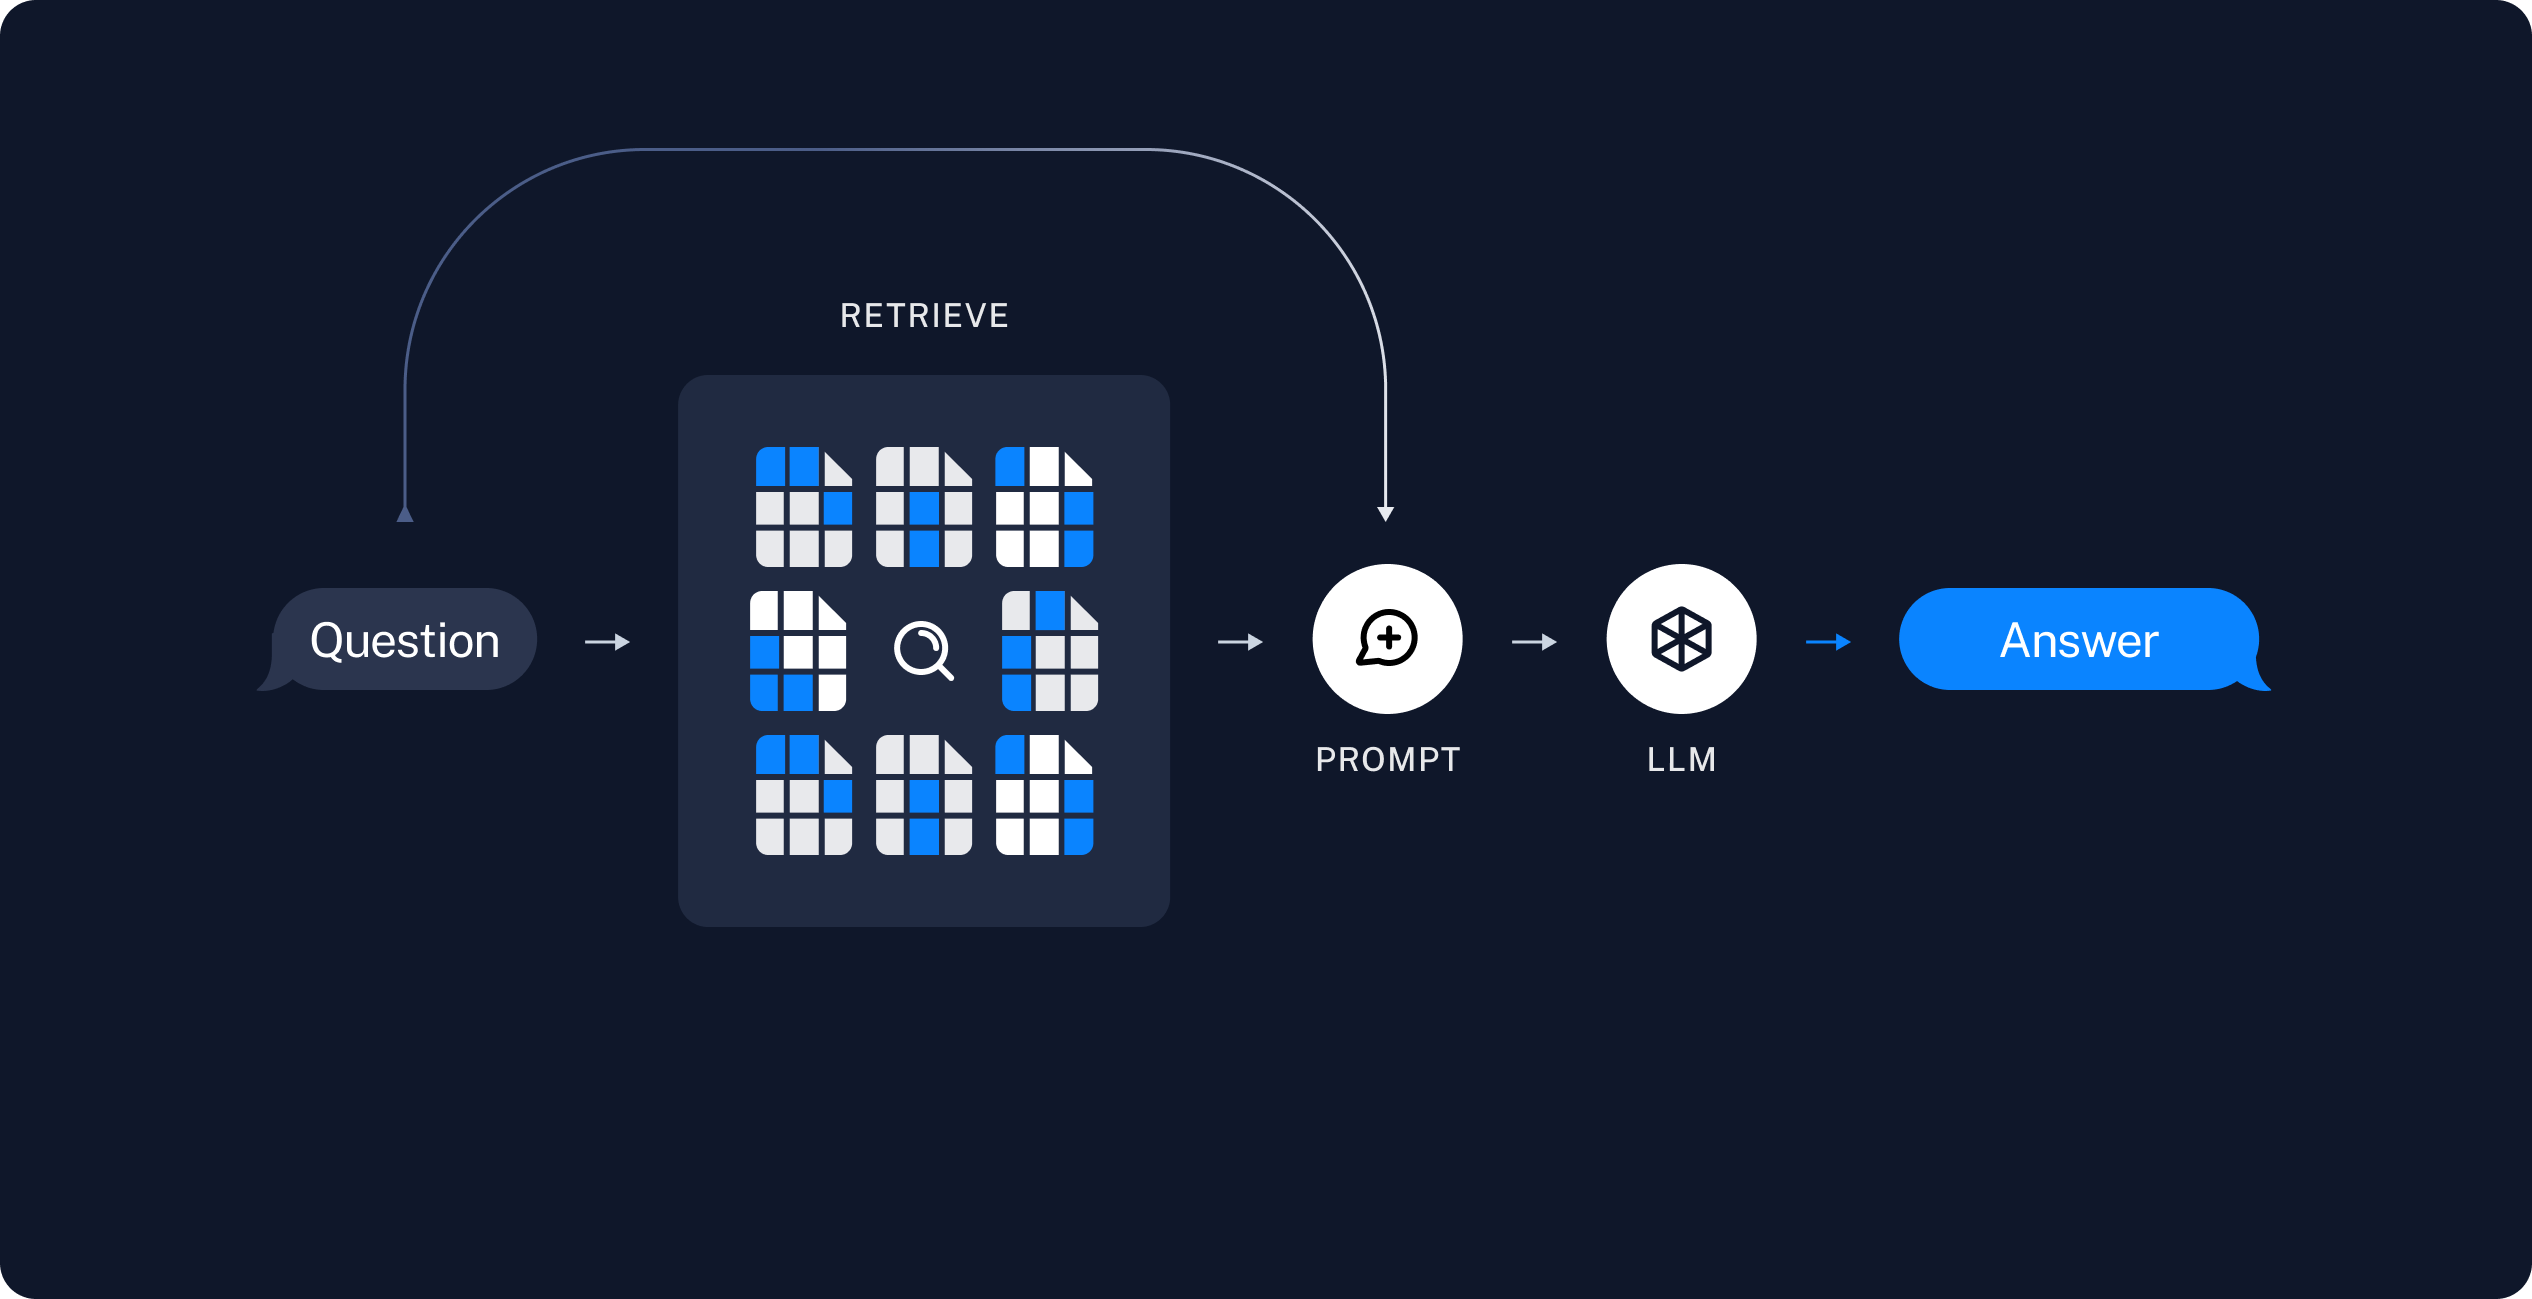
\includegraphics[width=0.75\textwidth]{images/lagchain-rag-retrieval.png}
    \caption{The retrieval phase: querying the vector store and invoking the LLM~\cite{langchain_rag}}
    \label{fig:retrieval_phase}
\end{figure}

\begin{enumerate}[label=\alph*.]
  \item \textbf{Context Retrieval:} The context retriever module follows a two-step process:
  \begin{enumerate}
    \item Embedding the user's query using the same embedding model employed during the embedding phase.
    \item Performing a similarity search in the vector database to identify top-matching chunks based on the embedded query.
  \end{enumerate}

  The quality of similarity search is crucial, as it directly impacts the relevance and accuracy of the LLM-generated response. In the embedding space, proximity denotes semantic similarity—closer vectors imply greater contextual relevance. However, efficient neighbor discovery in high-dimensional vector space is computationally expensive, and full database scans are often impractical \cite{sugawara2016approximately}.

  \item \textbf{Search Algorithms:} To balance accuracy, latency, and resource usage, the following approximate nearest neighbor (ANN) algorithms are commonly employed:
  \begin{enumerate}
    \item \textbf{Cosine Similarity Search:} Measures the cosine of the angle between vectors to determine their similarity. It is widely used in embedding-based retrieval tasks due to its scale invariance and intuitive geometric interpretation. 
    This is \textbf{highly parallelizable} and simple to implement. \cite{steck2024cosine}. 
    \textit{This is project primarily relies on cosine similarity for embedding retrieval.}
    
    \item \textbf{k-Nearest Neighbors (kNN):} A brute-force method that identifies the $k$ closest vectors through exhaustive comparisons~\cite{labelbox2023vectorsimilarity}.
    
    \textit{This project uses kNN as a fallback mechanism to search in the database using pg-vector}~\cite{pgvector}.

    \item \textbf{HNSW (Hierarchical Navigable Small World) Graphs:} Constructs a layered graph to enable fast traversal through neighbors across different granularity levels \cite{labelbox2023vectorsimilarity}.
    \item \textbf{ScaNN (Scalable Nearest Neighbors):} A Google-designed ANN method that integrates pruning, quantization, and partitioning for scalable, memory-efficient retrieval \cite{guo2020accelerating}.
  \end{enumerate}


\item \textbf{Output Generation:}
In this phase, the retrieved context and the user input—both in plain text form—are fed into the Large Language Model, as illustrated in Figure~\ref{fig:autoregressive_decoding}. The LLM processes the portion of input that fits within its context window and generates an output token. This token is then concatenated with the input and passed back to the LLM. The process repeats iteratively until the LLM produces an \textless{}EOS\textgreater{} (end-of-sequence) token.


\end{enumerate}

\subsection{Output Evaluation}
The evaluation of a Retrieval-Augmented Generation (RAG) system focuses on the quality of the output in terms of its relevance to the user's query and the information stored in the vector database. Since different components contribute uniquely to the overall performance, multiple metrics are used rather than a single aggregated score to allow for precise attribution and targeted optimization.

Classical metrics such as Precision, Recall, and F1 score, alongside NLP-specific metrics like ROUGE, are employed to assess performance. The evaluation considers several factors, as illustrated in Figure \ref{fig:RAGOutputevaluationmetrics}:
\begin{itemize}
    \item \textbf{Faithfulness, Output Relevance \& Semantic Similarity:} Measures the quality of the output relative to the input queries and retrieved context.
    \item \textbf{Context Recall \& Context Precision:} Assess the effectiveness of context retrieval and its utilization by the LLM.
\end{itemize}
\begin{figure}[H]
    \centering
    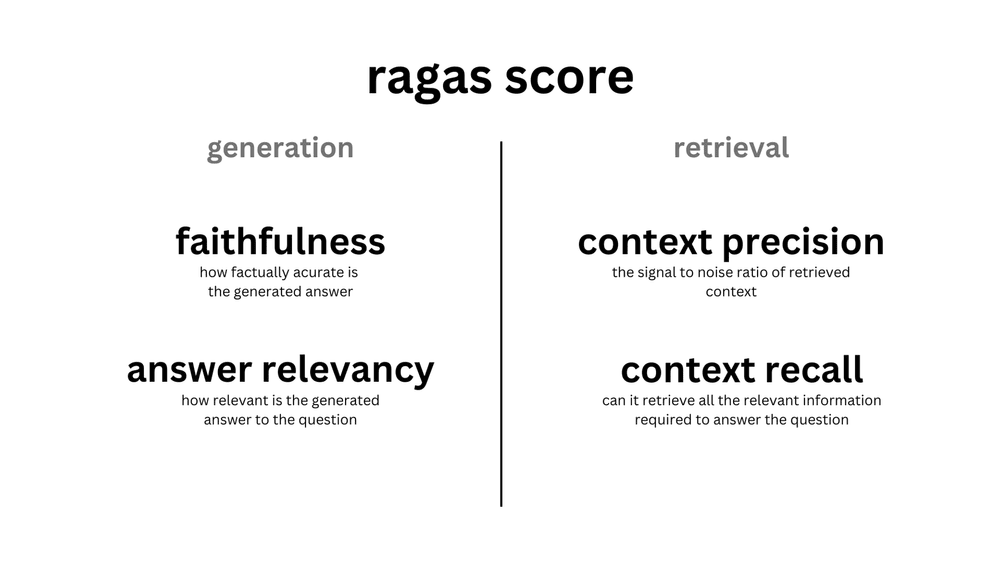
\includegraphics[width=0.56\linewidth]{images/rag-eval.png}
    \caption{RAG output evaluation metrics ~\cite{cardenas2023rag}}
    \label{fig:RAGOutputevaluationmetrics}
\end{figure}

